% Seed-42 split-sensitivity summary generated from
% results/split_sensitivity/cell_stratified_seed42_summary.csv.
\begin{figure*}[t]
  \centering
  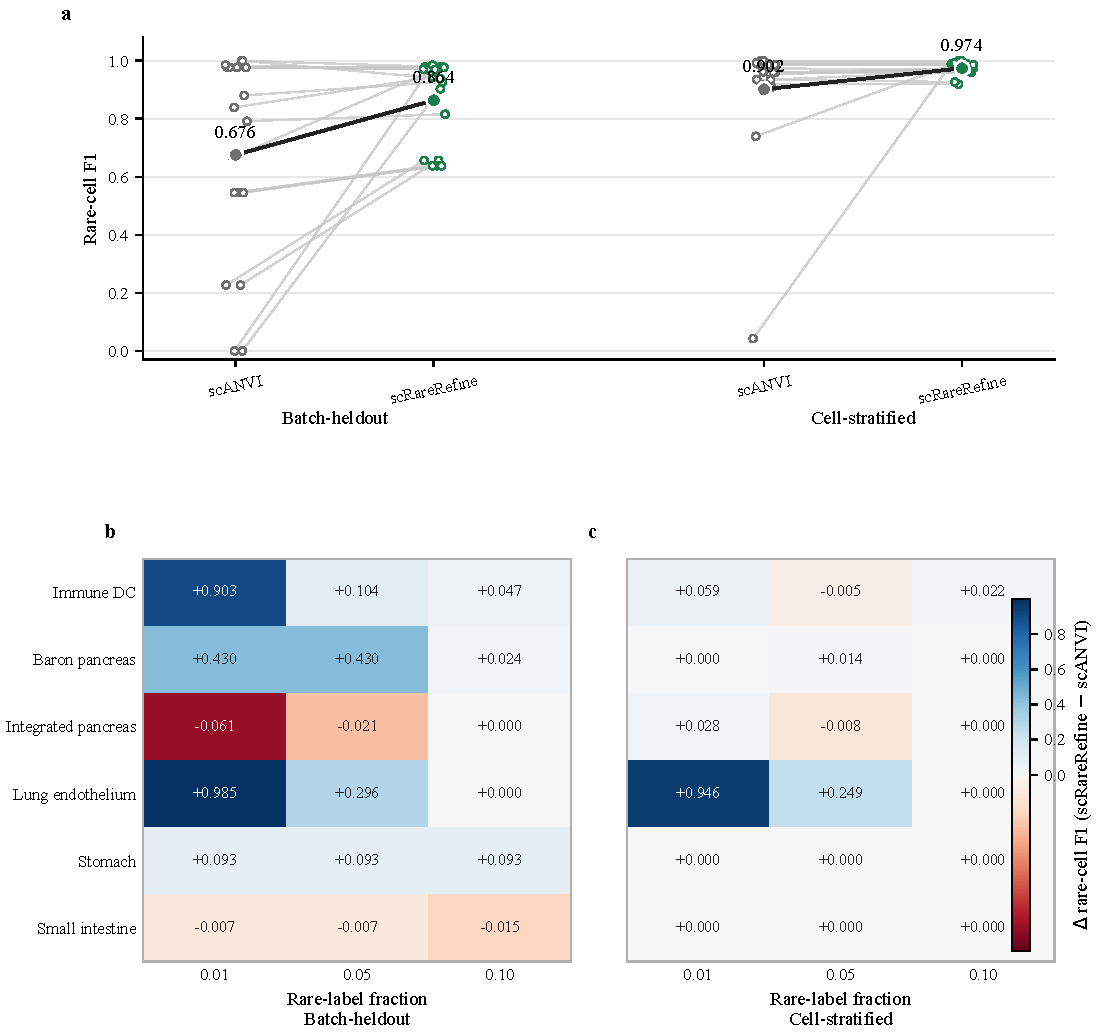
\includegraphics[width=0.95\textwidth]{results/split_sensitivity/split_sensitivity_seed42_summary.pdf}
  \caption{Split-sensitivity analysis for the six human datasets at seed 42.
  (a) Paired rare-cell F1 values for scANVI and scRareRefine across the 18
  dataset--budget units in the label-scarce region
  ($\mathrm{rare\_train\_size}\in\{0.01,0.05,0.10\}$); large markers denote
  descriptive means. (b,c) Per-unit F1 changes under batch-heldout and
  cell-stratified splitting. Cell-stratified splitting strengthens the scANVI
  backbone and reduces the average rescue opportunity, while preserving a
  positive mean scRareRefine gain; the annotated heatmaps retain all small
  negative and zero effects. This sensitivity experiment contains one seed and
  is separate from the multi-seed primary batch-heldout benchmark.}
  \label{fig:split-sensitivity-seed42}
\end{figure*}
